\documentclass[10pt,pdf,hyperref={unicode}]{beamer}

% \documentclass[aspectratio=43]{beamer}
% \documentclass[aspectratio=1610]{beamer}
% \documentclass[aspectratio=169]{beamer}

\usepackage{lmodern}
\usepackage{amsfonts}
\usepackage{amsmath}
% подключаем кириллицу 
\usepackage[T2A]{fontenc}
\usepackage[utf8]{inputenc}
\usepackage[russian]{babel}
% отключить клавиши навигации
\setbeamertemplate{navigation symbols}{}

% тема оформления
\usetheme{CambridgeUS}

% цветовая схема
\usecolortheme{spruce}

%Закругление выделений
\useinnertheme{rounded}

\useoutertheme[subsection=true]{miniframes}

\title{Моделирование образования сверхкоротких атмосферных разрядов под действием космических лучей}   
\subtitle{Обзорный доклад}
\author{Зелёный Михаил} 
\institute[ИЯИ]{Институт ядерных исследований РАН г. Троицк}
\date{\today}

%\logo{\includegraphics[height=5mm]{image/logo.png}\vspace{-7pt}}

\begin{document}

% титульный слайд
\begin{frame}
\titlepage
\end{frame} 


\begin{frame}
 	\begin{columns}
 		\column{0.5\textwidth}
 		\begin{center}
 		\includegraphics[width=0.3\paperwidth]{image/fig04.jpg}\\
 		Френкель Я. И.
 		\end{center} 
 			
 		\column{0.5\textwidth}
 		
 			\includegraphics[width=0.3\paperwidth]{image/fig05.jpg}\\
 			\begin{center}
 			Имянитов И. М.
            \end{center} 			 
 			
 	\end{columns}
\end{frame}


\begin{frame}
\begin{center}
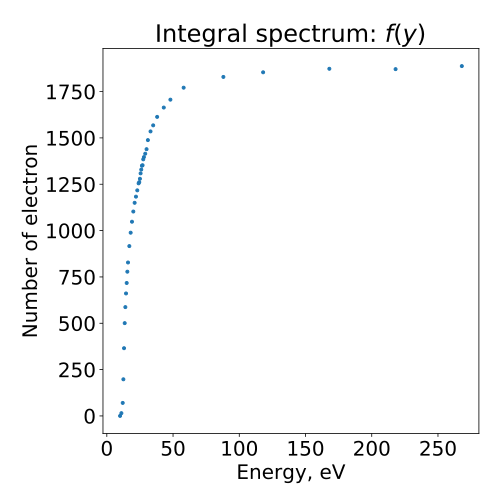
\includegraphics[width=0.6\paperwidth]{image/fig01.jpg}
\end{center}
\end{frame}
 


\begin{frame}
\frametitle{Terrestrial $\gamma$-ray flash (TGF)}
\begin{center}
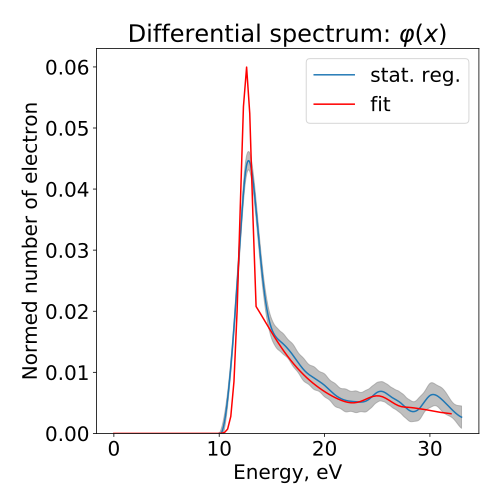
\includegraphics[width=0.8\paperwidth]{image/fig02.jpg}
\end{center}
\end{frame}


\begin{frame}
\frametitle{Нейтроны}
С энергией от тепловых до нескольких МэВ.
\begin{block}{Работы:}
\begin{itemize}
\item Shah G.N.//Nature[1985]
\item Chilingarian A,//Phys. Rev.[2010]
\item Более полный список в диссертации Дроздова А.Ю.
\end{itemize}
\end{block}
\end{frame}

\begin{frame}
\frametitle{Пробой на убегающих электронах}
\begin{center}
\includegraphics[width=0.6\paperwidth]{image/fig06.png}
\end{center}
\end{frame}


\begin{frame}
\frametitle{Образование положительной обратной связи}
\begin{block}{Физические процессы}
\begin{itemize}
\item Высоконергетичные: ионизация, тормозное излучение, распространение гамма-квантов...
\item Низкоэнергитичные: рекомбинация, прилипания, рассеяние на атомных уровнях, характеристическое излучение...
\end{itemize}
\end{block}
\begin{block}{Возможные механизмы}
\begin{itemize}
\item Обратное распространения гамма-квантов?
\item Разворот электронов?
\item Цепочка гамма-электроных столкновений?
\item Транспорт гамма-квантов в слоистых полевых структурах?
\item Позитроны???
\end{itemize}
\end{block}
\end{frame}

\begin{frame}
\frametitle{Geant4 low energy}
\begin{block}{PENELOPA}
\begin{itemize}
\item Пороги рождения частиц $\sim$10 КэВ
\item Более полный набор взаимодействия
\end{itemize}
\end{block}
\begin{block}{Livermore}
\begin{itemize}
\item Более низкие пороги (до $\sim$5 эВ)
\item Нестабильная работа, обнаружены ошибки при трекинге
\end{itemize}
\end{block}
\end{frame}

\begin{frame}
\frametitle{Прохождение электронов в газе}
\begin{block}{Рекомбинация}
\begin{itemize}
\item Неясен доминирующий механизм
\item В электрических полях считается малой, но нет количесвенного описания
\item Неизмерены сечения в нужных диапазонах
\end{itemize}
\end{block}
\Large{Имеются противоречивые данные по гасящим способностям газов}
\end{frame}

\begin{frame}
\begin{center}
\Large{Спасибо за внимание}
\end{center}
\end{frame}

\end{document}